% ----------------------- TODO ---------------------------
% Diese Daten müssen pro Blatt angepasst werden:
\newcommand{\NUMBER}{3}
\newcommand{\EXERCISES}{5}
% Diese Daten müssen einmalig pro Vorlesung angepasst werden:
\newcommand{\COURSE}{Grundlagen der Digitaltechnik}
\newcommand{\TOPIC}{Registerschaltungen}
\newcommand{\DATE}{06.05.2022}
% ----------------------- TODO ---------------------------

\documentclass[a4paper]{scrartcl}

\usepackage[utf8]{inputenc}
\usepackage[ngerman]{babel}
\usepackage{amsmath}
\usepackage{amssymb}
\usepackage{fancyhdr}
\usepackage{color}
\usepackage{graphicx}
\usepackage{lastpage}
\usepackage{listings}
\usepackage{tikz}
\usepackage{pdflscape}
\usepackage{subfigure}
\usepackage{float}
\usepackage{polynom}
\usepackage{hyperref}
\usepackage{tabularx}
\usepackage{forloop}
\usepackage{geometry}
\usepackage{listings}
\usepackage{fancybox}
\usepackage{tikz}
\usepackage{algpseudocode,algorithm,algorithmicx}

%Definiere Let-Command für algorithmen
\newcommand*\Let[2]{\State #1 $\gets$ #2}

\input kvmacros

%Größe der Ränder setzen
\geometry{a4paper,left=3cm, right=3cm, top=3cm, bottom=3cm}

%Kopf- und Fußzeile
\pagestyle {fancy}
\fancyhead[L]{\COURSE}
\fancyhead[R]{\DATE}

\fancyfoot[L]{}
\fancyfoot[C]{}
\fancyfoot[R]{Seite \thepage /\pageref*{LastPage}}
\setlength{\parindent}{0pt}

%Formatierung der Überschrift, hier nichts ändern
\def\header#1#2{
  \begin{center}
    {\Large Labor #1: \TOPIC}\\
    {(Datum #2)}
  \end{center}
}


\begin{document}


\header{Nr. \NUMBER}{\DATE}

\section*{Aufgabe 1: Registerschaltungen}
\subsection*{a) Register}
Lege ein Subsystem an und baue in Logisim ein 8-Bit Register mit Hilfe von D-Flipflops (nutze D-Flipflops und nicht den Registerbaustein von Logisim) auf. 
Neben dem 8-Bit Ein- und Ausgang soll das Register einen Clock Eingang besitzen, sowie einen asynchronen Reseteingang.
Funktion:
\begin{itemize}
  \item Bei steigender Taktflanke sollen die Eingangsbits übernommen werden
  \item Bei 1 am Reset sollen asynchron alle Bits zurückgesetzt werden
\end{itemize}


  \begin{figure}[h]
    \centering
    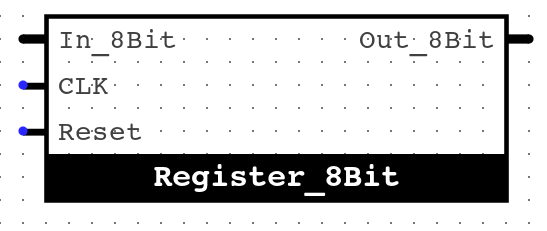
\includegraphics[width=5cm]{Reg.png}
  \end{figure}

  
\subsection*{b) Schieberegister}
\subsubsection*{i) Design}
Lege ein Subsystem an und baue in Logisim ein 8-Bit Schieberegister mit Flipflops und Logik auf. Das Schieberegister soll 
jeweils einen seriellen sowie einen parallelen Ein- und Ausgang haben. Mit einem Steuerbit soll zwischen Shift=0 und Load=1
umgestellt werden. Im Shift Mode sollen die Bits zusammen mit einer Taktflanke geschoben werden. Im Load Mode sollen die Eingänge 
am parallelen Eingang asynchron übernommen werden. Außerdem soll es ein Reset-Eingang geben,
welcher das Register asynchron reseted. Es ist ausreichend, wenn das Register
nach links schieben kann.

\textbf{Hinweis:} Die D-Flipflops in Logisim besitzen einen asynchronen Set/Reset-Eingang.


\begin{figure}[h]
  \centering
  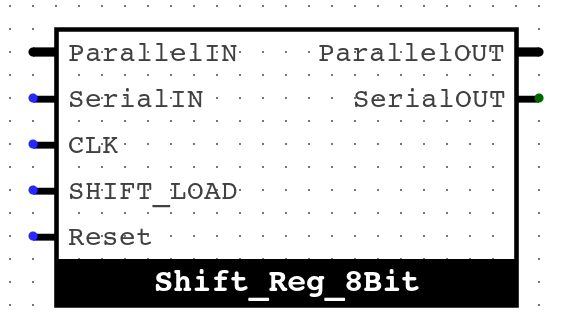
\includegraphics[width=5cm]{ShiftReg.png}
\end{figure}

\subsubsection*{ii) Test}
Lege ein weiteres Subsystem - Test\_Schieberegister - an und teste die Funktion des Schieberegisters.
Teste ob:
\begin{itemize}
  \item Im Shift-Mode (shift + clk):
  \begin{itemize}
    \item die Bits am Ausgang richtig verschoben werden
    \item der serielle Eingang ``reingeschoben'' wird
  \end{itemize} 
  \item Im Load-Mode der parallele Eingang direkt (asynchron) übernommen wird
  \item Beim Reset direkt (asynchron) alle Bits zurückgesetzt werden
\end{itemize}

\section*{Aufgabe 2: Kommunikationssystem}
Die Register und Schieberegister aus Aufgabe 1 sollen jetzt zur Realisierung eines Master/Slave Bussystems genutzt werden. Dieses soll aus einem Master 
und zwei Slaves bestehen. Um es einfacher zu halten, kann der Master nur senden und die Slaves nur empfangen. Das Bussystem soll aus gemeinsamen
einem Takt-Signal (Clk),
einem gemeinsamen Datensignal, sowie aus Select-Leitungen bestehen. Mit der Select-Leitung wählt der Master den Slave aus, mit welchem er kommunizieren will.
Auf dem synchronen Bus soll mit jeder positiven Flanke am Takteingang das aktuell anliegende Daten Bit übernommen werden, aber nur wenn der Slave ausgewählt ist
(Select-Leitung).

\subsection*{a) Master-Baustein}
Lege ein Subsystem an und baue den Master-Baustein auf. Der Master hat folgende Eingänge:
\begin{itemize}
  \item 8-Bit Dateneingang
  \item Set-Eingang: Mit positiver Flanke am Set-Eingang soll der 8-Bit Dateneingang ins interne Register übernommen werden
  \item Clk: der Bus-Takteingang (Clock-Signal des Buses), mit jeder Flanke am Clk soll ein  Bit aus dem internen Register versendet werden
  \item 1-Bit Select: Bei ``0'' soll Slave0 der Empfänger sein, bei ``1'' Slave1
  \item Reset: Eingang, welcher alle intern gespeicherten ``Sachen'' reseted
\end{itemize}
Der Ausgang des Masters soll mit den Eingängen der Slaves verschaltet werden. Folgende Ausgänge soll es geben.
\begin{itemize}
  \item 1-Bit Data-Out: Mit jeder Clk-Flanke soll das ``hinterste'' Bit im internen Schieberegister auf den Bus geschoben werden.
  \item Slave-Select 0: High, wenn 0 am Select Eingang
  \item Slave-Select 1: High, wenn 1 am Select Eingang
\end{itemize}
\textbf{Hinweis:}
Das Schieberegister, Pins und Logikgates sollten ausreichen, um diese Schaltung zu realisieren.

\begin{figure}[h]
  \begin{center}
  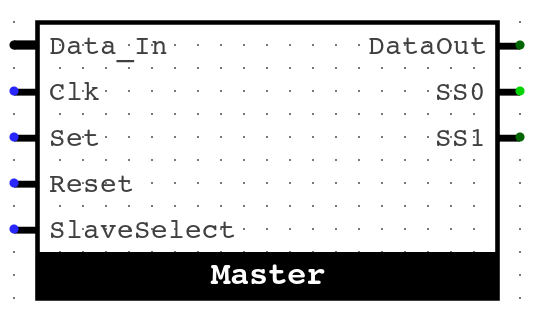
\includegraphics[width=5cm]{Master.png}
\end{center}
\end{figure}

\subsection*{b) Slave-Baustein}
Lege ein Subsystem an und baue den Slave-Baustein auf. Der Slave hat folgende Eingänge:
\begin{itemize}
  \item 1-Bit Data-In: der Dateneingang
  \item Clk: der Bus-Takteingang (Clock-Signal des Buses), mit jeder Flanke am Clk soll ein Bit empfangen werden
  \item Select: Nur wenn der Select-Eingang ``1'' ist, soll auf Data-In und Clk reagiert werden (enable).
  \item Reset: Eingang, welcher alle intern gespeicherten ``Sachen'' reseted
  \item Reset Data-Ready: Über diesen Eingang soll das Data-Ready Flag zurückgesetzt werden
\end{itemize}
Ausgaben soll der Slave lediglich tätigen, wenn ein ganzes Byte Empfangen wurde. Er soll folgende Ausgänge haben:
\begin{itemize}
  \item 8-Bit Data-Out: Ausgabe des letzten empfangenen Byte. Das vorherige Byte soll solange anliegen bis ein neues empfangen wurde. Der Ausgang
  ändert sich daher nur mit dem 8., 16., 24. ... empfangenen Bit.
  \item Data-Ready: Data Ready soll auf ``1''
   gesetzt werden, sobald 8 Bit empfangen wurden. Es soll anzeigen, das ein neues Byte angekommen ist. Es wird asynchron über Reset Data-Ready zurückgesetzt.
\end{itemize}


\textbf{Hinweise:}
\begin{itemize}
 \item Neben dem Register und Schieberegister aus Aufgabe 1 wird für dieses Subsystem auch ein Counter, welcher auf 8 zählen kann, benötigt. Dieser kann aus
  der Logisim Bibliothek benutzt werden.
  \item Die empfangenen Bits sollen in ein Schieberegister geschoben werden, wenn 8-Bits empfangen wurden, soll der Zustand
  des Schieberegisters in einem zweiten ``normalen'' Register übernommen
  werden.
  \item Ein 3-Bit Counter kann verwendet werden um mitzuzählen, wie viele Bits bereits empfangen wurden.
  \item Die Implementierung des Data-Ready Signals ist etwas tricky. Das Data-Ready soll nach 8 empfangenen Bits auf High gehen.  
  Dies bedeutet, der interne Counter, welcher die Datenbits zählt steht in diesem Zustand auf 0 (der zählt von 0 - 7).
  Da Data-Ready aber z.B. nach einem Reset nicht auf high stehen soll, da noch gar nichts empfangen wurde, kann man dies nicht direkt verknüpfen.
  Lösen kann man das Problem in dem man zusätzlich noch das ``3CT'' 
  Singal des Counters betrachtet, dies wird für einen Takt ``high'', wenn der Counter seinen maximalen Wert (7) erreicht.
  \item Vermutlich ist trotz des obigen Hinweises, die Implementierung des Data-Ready Signals immer noch etwas tricky, falls man hier feststeckt kann man 
  dies auch weglassen.
\end{itemize}


\begin{figure}[h]
\centering
  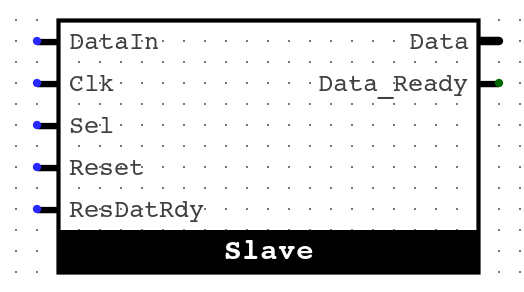
\includegraphics[width=5cm]{Slave.png}
\end{figure}


\subsection*{c) Assembly \& Test}
\subsubsection*{i) Design}
Zur Überprüfung der Funktion soll jetzt das Bussystem aus einem Master und zwei Slave Instanzen 
zusammen gebaut werden. Durch das Auswahlbit sollen entweder Daten vom Master an Slave0 oder Slave1 geschickt werden.

Der Data-Out des Masters und die Data-In der Slaves sollen miteinander verbunden werden, sie stellen die Datenleitung dar.
Die Bus-Clk aller drei Bausteine sollen mit einem Clk-Baustein verbunden werden und die Slave-Select Signale des Masters
sollen die Slaves auswählen (enablen)

Die restlichen Ein- und Ausgänge sollen User-Input oder Output darstellen. Benutze geeignete Input/Output Elemente von Logisim. Falls du nicht 
weiterkommst, ist auf der letzten Seite ein Referenzdesign. 

\subsubsection*{ii) Test}
Teste das Bussystem. Bei korrekter Funktion sollte sich das System wie folgt verhalten:
\begin{enumerate}
  \item Drücke Reset, um einen definierten Zustand herzustellen
  \begin{itemize}
    \item Alle Datenausgänge der Slaves, sowie das interne Register des Masters sollten nun 0 sein.
  \end{itemize}
  \item Stelle am Data-In des Masters eine gewünschtes Byte ein, welches übertragen werden soll
  \item Drücke Set-Data, um die Daten in den Master zu schreiben
  \item Wähle am Slave-Select den gewünschten Slave aus
  \item Toggle den Clk-Baustein, sodass es 8 Cycles gibt (8 positive Flanken)
  \item Resultat:
  \begin{itemize}
    \item Am Datenausgang des ausgewählten Slaves sollten nun die eingestellten Daten angekommen sein 
    \item Das Data-Ready Signal sollte auf high gesprungen sein
  \end{itemize}
  \item Toggle den Clk-Baustein ein weiteres Mal
  \item Resultat:
  \begin{itemize}
    \item An den Ausgängen des Slaves sollte sich nichts verändert haben
  \end{itemize}
  \item Drücke Reset Data-Ready
  \item Resultat:
  \begin{itemize}
    \item Das Data-Ready sollte zurückgesetzt worden sein
  \end{itemize}
  \item Wiederhole den Test mit dem anderen Slave
  \item Drücke in einem beliebigem Zustand den Reset-Knopf und schaue, ob alles korrekt reseted wird.
\end{enumerate}


\subsection*{d) Erklärungen}
Hier sollen noch ein paar erklärende Hinweise zur Übung gegeben werden.\\
Das simulierte Bussystem ist lose an das Bussystem SPI (Serial Peripheral Interface) angelehnt. Im folgenden werden noch ein paar Fragen erläutert, die 
vllt. aufgekommen sind:
\begin{itemize}
  \item Was soll die Aufgabe grundsätzlich darstellen?\\
  Die simulierte Schaltung soll ein vereinfachtes SPI Interface von z.B. drei Microcontrollern darstellen. Dieses Bus-Interface ist dabei ein Teil des Controllers.
  Die Eingänge des Masters  werden von der CPU
  des Master-$\mu$C angsteuert. Über den Bus soll der Master-$\mu$C dann Daten an die beiden Slave-$\mu$Cs senden können. Der Datenausgang der Slave-Bausteine kann dann
  wiederrum von der CPU des Slave-Controllers verarbeitet werden.
  \item Warum benutzt man überall einen asynchronen Reset?\\
  Um zu einem Zeitpunkt x, z.B. start des System einen definierten Zustand zu erreichen, müssen alle Register zurückgesetzt werden können. Dies wird erreicht durch 
  den Reset. Dies ist im Prinzip genau das gleiche wie der Reset Pin eines $\mu$Cs.
  \item Warum braucht man das Data-Ready Signal?\\
  Wenn man diese Schaltung als Teil eines größeren Systems (z.B. $\mu$C) sieht, könnte man das Data-Ready Signal als Interrupt-Signal verwenden. Dadurch wird
  der Controller notifiziert so bald es neue Daten gibt. Darauf muss das Program des Controllers dann reagieren.
  \item Warum braucht man das Reset Data-Ready Signal?\\
  Sobald die Microcontroller Software die Daten ``gesehen'' hat, setzt es das Data-Ready zurück, um beim nächsten Empfang wieder einen Interrupt zu erhalten.
  \item Warum kann man hier nur in eine Richtung senden?\\
  Dies wurde so entschieden, um die Schaltung nicht noch komplizierter zu machen.
\end{itemize}





\section*{Aufgabe 3: Bonus (wenn Zeit übrig)}
Bei der Analyse der ALU aus Aufgabenblatt 2 ist aufgefallen, dass die erstellte ALU keine Operation für eine 
Rechtsverschiebung zur Verfügung stellt, obwohl dies eigentlich zur Minimalfunktion einer ALU gehört. Entwickle eine 
Schaltnetz, welches die Rechtsverschiebung durchführt, teste dieses und füge es inder ALU hinzu.\\
Müssen noch andere Sachen erweitert aus der neuen Teilschaltung hinzugefügt werden?
\\

\textbf{Hinweis:} 
\begin{itemize}
  \item Rechtsverschiebung bedeutet, dass unterste 8-Bits "weggeschoben" wird und alle anderen Bits eine Stelle nach unten rücken:\\
  Bsp.: $0b1001 \rightarrow 0b0100$
  \item Schaltnetz bedeutet das hier lediglich Logik, aber keine speicherenden Elemente (Flipflops) benutzt werden sollen.
\end{itemize}

\section*{Appendix}
\begin{figure}[h]
  \centering
  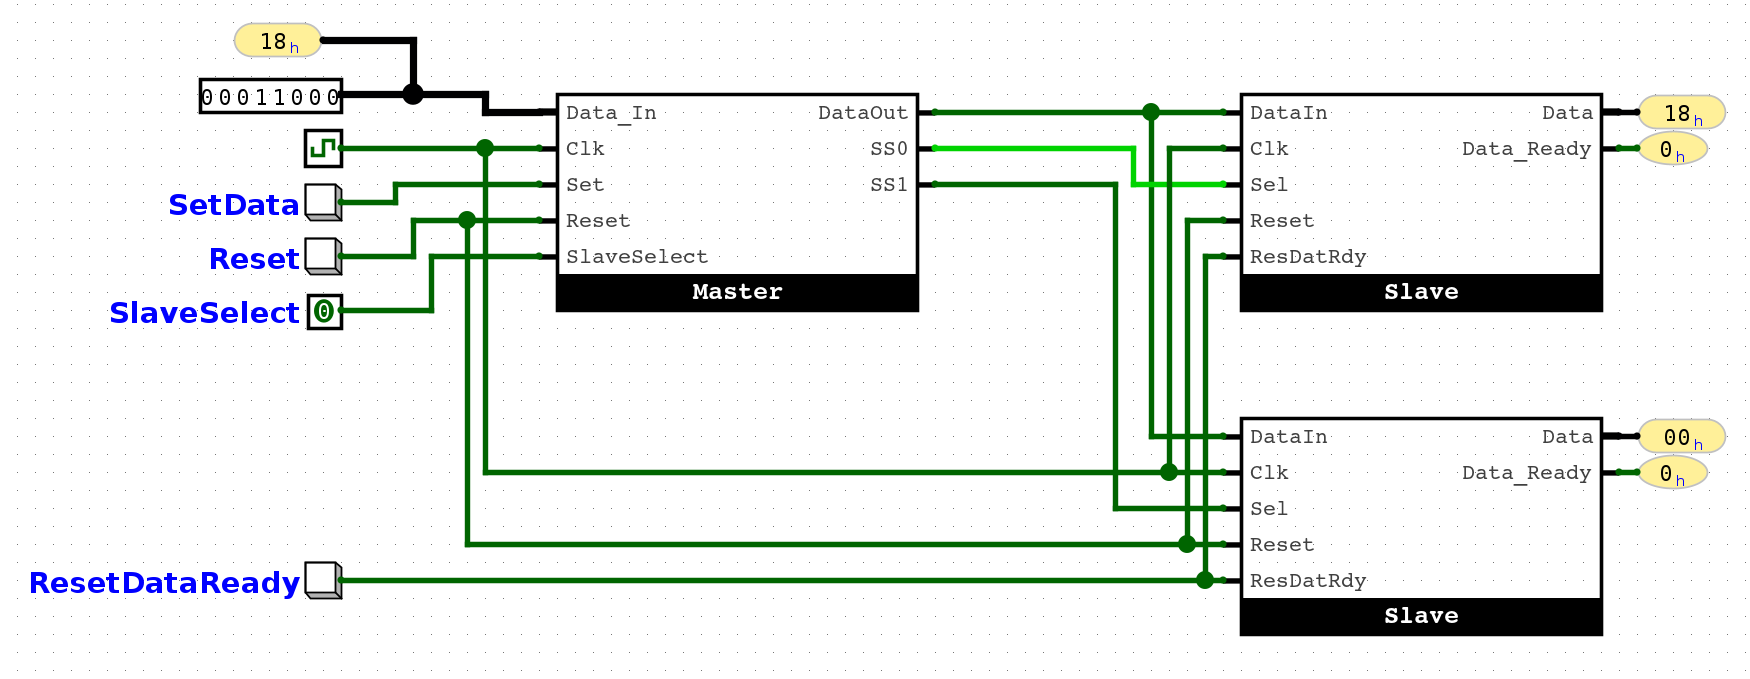
\includegraphics[width=\textwidth]{Assembly.png}
\end{figure}

  
\end{document}
%%% Local Variables:
%%% mode: latex
%%% TeX-master: t
%%% End: